% Options for packages loaded elsewhere
% Options for packages loaded elsewhere
\PassOptionsToPackage{unicode}{hyperref}
\PassOptionsToPackage{hyphens}{url}
\PassOptionsToPackage{dvipsnames,svgnames,x11names}{xcolor}
%
\documentclass[
  letterpaper,
  DIV=11,
  numbers=noendperiod]{scrartcl}
\usepackage{xcolor}
\usepackage{amsmath,amssymb}
\setcounter{secnumdepth}{5}
\usepackage{iftex}
\ifPDFTeX
  \usepackage[T1]{fontenc}
  \usepackage[utf8]{inputenc}
  \usepackage{textcomp} % provide euro and other symbols
\else % if luatex or xetex
  \usepackage{unicode-math} % this also loads fontspec
  \defaultfontfeatures{Scale=MatchLowercase}
  \defaultfontfeatures[\rmfamily]{Ligatures=TeX,Scale=1}
\fi
\usepackage{lmodern}
\ifPDFTeX\else
  % xetex/luatex font selection
\fi
% Use upquote if available, for straight quotes in verbatim environments
\IfFileExists{upquote.sty}{\usepackage{upquote}}{}
\IfFileExists{microtype.sty}{% use microtype if available
  \usepackage[]{microtype}
  \UseMicrotypeSet[protrusion]{basicmath} % disable protrusion for tt fonts
}{}
\makeatletter
\@ifundefined{KOMAClassName}{% if non-KOMA class
  \IfFileExists{parskip.sty}{%
    \usepackage{parskip}
  }{% else
    \setlength{\parindent}{0pt}
    \setlength{\parskip}{6pt plus 2pt minus 1pt}}
}{% if KOMA class
  \KOMAoptions{parskip=half}}
\makeatother
% Make \paragraph and \subparagraph free-standing
\makeatletter
\ifx\paragraph\undefined\else
  \let\oldparagraph\paragraph
  \renewcommand{\paragraph}{
    \@ifstar
      \xxxParagraphStar
      \xxxParagraphNoStar
  }
  \newcommand{\xxxParagraphStar}[1]{\oldparagraph*{#1}\mbox{}}
  \newcommand{\xxxParagraphNoStar}[1]{\oldparagraph{#1}\mbox{}}
\fi
\ifx\subparagraph\undefined\else
  \let\oldsubparagraph\subparagraph
  \renewcommand{\subparagraph}{
    \@ifstar
      \xxxSubParagraphStar
      \xxxSubParagraphNoStar
  }
  \newcommand{\xxxSubParagraphStar}[1]{\oldsubparagraph*{#1}\mbox{}}
  \newcommand{\xxxSubParagraphNoStar}[1]{\oldsubparagraph{#1}\mbox{}}
\fi
\makeatother


\usepackage{longtable,booktabs,array}
\usepackage{calc} % for calculating minipage widths
% Correct order of tables after \paragraph or \subparagraph
\usepackage{etoolbox}
\makeatletter
\patchcmd\longtable{\par}{\if@noskipsec\mbox{}\fi\par}{}{}
\makeatother
% Allow footnotes in longtable head/foot
\IfFileExists{footnotehyper.sty}{\usepackage{footnotehyper}}{\usepackage{footnote}}
\makesavenoteenv{longtable}
\usepackage{graphicx}
\makeatletter
\newsavebox\pandoc@box
\newcommand*\pandocbounded[1]{% scales image to fit in text height/width
  \sbox\pandoc@box{#1}%
  \Gscale@div\@tempa{\textheight}{\dimexpr\ht\pandoc@box+\dp\pandoc@box\relax}%
  \Gscale@div\@tempb{\linewidth}{\wd\pandoc@box}%
  \ifdim\@tempb\p@<\@tempa\p@\let\@tempa\@tempb\fi% select the smaller of both
  \ifdim\@tempa\p@<\p@\scalebox{\@tempa}{\usebox\pandoc@box}%
  \else\usebox{\pandoc@box}%
  \fi%
}
% Set default figure placement to htbp
\def\fps@figure{htbp}
\makeatother





\setlength{\emergencystretch}{3em} % prevent overfull lines

\providecommand{\tightlist}{%
  \setlength{\itemsep}{0pt}\setlength{\parskip}{0pt}}



 
\usepackage[]{natbib}
\bibliographystyle{plainnat}


\usepackage{booktabs}
\usepackage{longtable}
\usepackage{array}
\usepackage{multirow}
\usepackage{wrapfig}
\usepackage{float}
\usepackage{colortbl}
\usepackage{pdflscape}
\usepackage{tabu}
\usepackage{threeparttable}
\usepackage{threeparttablex}
\usepackage[normalem]{ulem}
\usepackage{makecell}
\usepackage{xcolor}
\KOMAoption{captions}{tableheading}
\makeatletter
\@ifpackageloaded{caption}{}{\usepackage{caption}}
\AtBeginDocument{%
\ifdefined\contentsname
  \renewcommand*\contentsname{Table of contents}
\else
  \newcommand\contentsname{Table of contents}
\fi
\ifdefined\listfigurename
  \renewcommand*\listfigurename{List of Figures}
\else
  \newcommand\listfigurename{List of Figures}
\fi
\ifdefined\listtablename
  \renewcommand*\listtablename{List of Tables}
\else
  \newcommand\listtablename{List of Tables}
\fi
\ifdefined\figurename
  \renewcommand*\figurename{Figure}
\else
  \newcommand\figurename{Figure}
\fi
\ifdefined\tablename
  \renewcommand*\tablename{Table}
\else
  \newcommand\tablename{Table}
\fi
}
\@ifpackageloaded{float}{}{\usepackage{float}}
\floatstyle{ruled}
\@ifundefined{c@chapter}{\newfloat{codelisting}{h}{lop}}{\newfloat{codelisting}{h}{lop}[chapter]}
\floatname{codelisting}{Listing}
\newcommand*\listoflistings{\listof{codelisting}{List of Listings}}
\makeatother
\makeatletter
\makeatother
\makeatletter
\@ifpackageloaded{caption}{}{\usepackage{caption}}
\@ifpackageloaded{subcaption}{}{\usepackage{subcaption}}
\makeatother
\usepackage{bookmark}
\IfFileExists{xurl.sty}{\usepackage{xurl}}{} % add URL line breaks if available
\urlstyle{same}
\hypersetup{
  pdftitle={Wide Bay Seagrass Resilience Modeling},
  pdfauthor={Michael Dumelle (Dumelle Consulting); Erin E. Peterson (EP Consulting)},
  colorlinks=true,
  linkcolor={blue},
  filecolor={Maroon},
  citecolor={Blue},
  urlcolor={Blue},
  pdfcreator={LaTeX via pandoc}}


\title{Wide Bay Seagrass Resilience Modeling}
\usepackage{etoolbox}
\makeatletter
\providecommand{\subtitle}[1]{% add subtitle to \maketitle
  \apptocmd{\@title}{\par {\large #1 \par}}{}{}
}
\makeatother
\subtitle{DRFA 21/22 Biodiversity Conservation Marine Final Report
Project}
\author{Michael Dumelle (Dumelle Consulting) \and Erin E. Peterson (EP
Consulting)}
\date{2026-05-11}
\begin{document}
\maketitle

\renewcommand*\contentsname{Table of contents}
{
\hypersetup{linkcolor=}
\setcounter{tocdepth}{3}
\tableofcontents
}

\section{Introduction}\label{introduction}

Over the past few decades, various scientific studies have informed our
current understanding of trends, behaviors, and flood responses of
seagrass cover in Wide Bay
\citep{preen1995flood, mcmahon2005herbicide, york2022post} as well as
Australia more widely
\citep{kilminster2015unravelling, gilby2018seagrass, o2018seagrass}.
Remote sensing has offered new capabilities for seagrass cover mapping
\citep{roelfsema2009integrated}, while innovative statistical approaches
have offered novel methods for studying resilience at site-specific
scales \citep{gilby2023drivers}. Our work adds to this body of
literature by applying spatially explicit statistical models
\citep{cressie1993statistics} to study the drivers, resilience, and
recovery of total percent seagrass cover in Wide Bay and Moreton Bay
\citep{dumelle2026moreton}. Specifically, we provide and contextualize
answers to three specific research questions, applicable to Wide Bay:

\begin{enumerate}
\def\labelenumi{\arabic{enumi}.}
\tightlist
\item
  Can we identify water quality covariates that act as triggers for
  seagrass cover management responses? Are these triggers different
  based on whether they result from a specific event (e.g., flood) or
  ambient conditions?
\item
  Did seagrass cover improve after the flood event(s)? If so, how and
  where?
\item
  Can we identify site-specific resilience indicators, which describe
  where recovery is likely to be enhanced or impeded? If so, what
  factors contribute to seagrass resilience?
\end{enumerate}

\section{Seagrass Cover Model}\label{seagrass-cover-model}

\subsection{Data}\label{data}

The seagrass cover dataset was provided by EcoFutures Consulting. It
included nearly 4000 seagrass cover observations in Wide Bay across
several financial years (1998-1999, 1999-2000, 2000-2001, 2001-2002,
2021-2022, 2022-2023, and 2023-2024). The data from 1998-2002 were
omitted as they were distant temporally and did not have corresponding
eReefs water-quality data \citep{steven2019ereefs}. Thus we proceed with
a subset of 2663 observations for modeling. Of the 2663 observations,
1073 were in 2021-2022, 524 were in 2022-2023, and 1066 were in
2023-2024 (Table~\ref{tbl-n_fy_wb}). There were four seagrass species
found in the dataset: \emph{Halophila decipiens} (HD), \emph{Halophila
spinulosa} (HS), \emph{Halophila ovalis} (HO), \emph{Halodule uninervis}
/ \emph{Zostera muelleri} (ZMHU).

\begin{table}

\caption{\label{tbl-n_fy_wb}The sample size and percent of total sample
size for total percent seagrass cover observations in Wide Bay, by
financial year.}

\centering{

\centering
\begin{tabular}{lrl}
  \toprule
Financial Year & Sample Size & Percent of Total \\ 
  \midrule
2021-2022 & 1073.00 & 40.3\% \\ 
  2022-2023 & 524.00 & 19.7\% \\ 
  2023-2024 & 1066.00 & 40.0\% \\ 
  Total & 2663.00 & 100.0\% \\ 
   \bottomrule
\end{tabular}

}

\end{table}%

Seagrass cover is a percentage that ranges from 0 (no seagrass) to 100
(complete seagrass cover). Figure~\ref{fig-cover_fy_wb} shows total
cover by financial year throughout the Bay. Total cover tends to be
highest near the eastern shoreline of the Bay and lowest in the middle
of the Bay. Note that 2022-2023 contained the fewest number of samples,
lacking significant samples in the Great Sandy Strait compared to the
other years.

\begin{figure}

\centering{

\pandocbounded{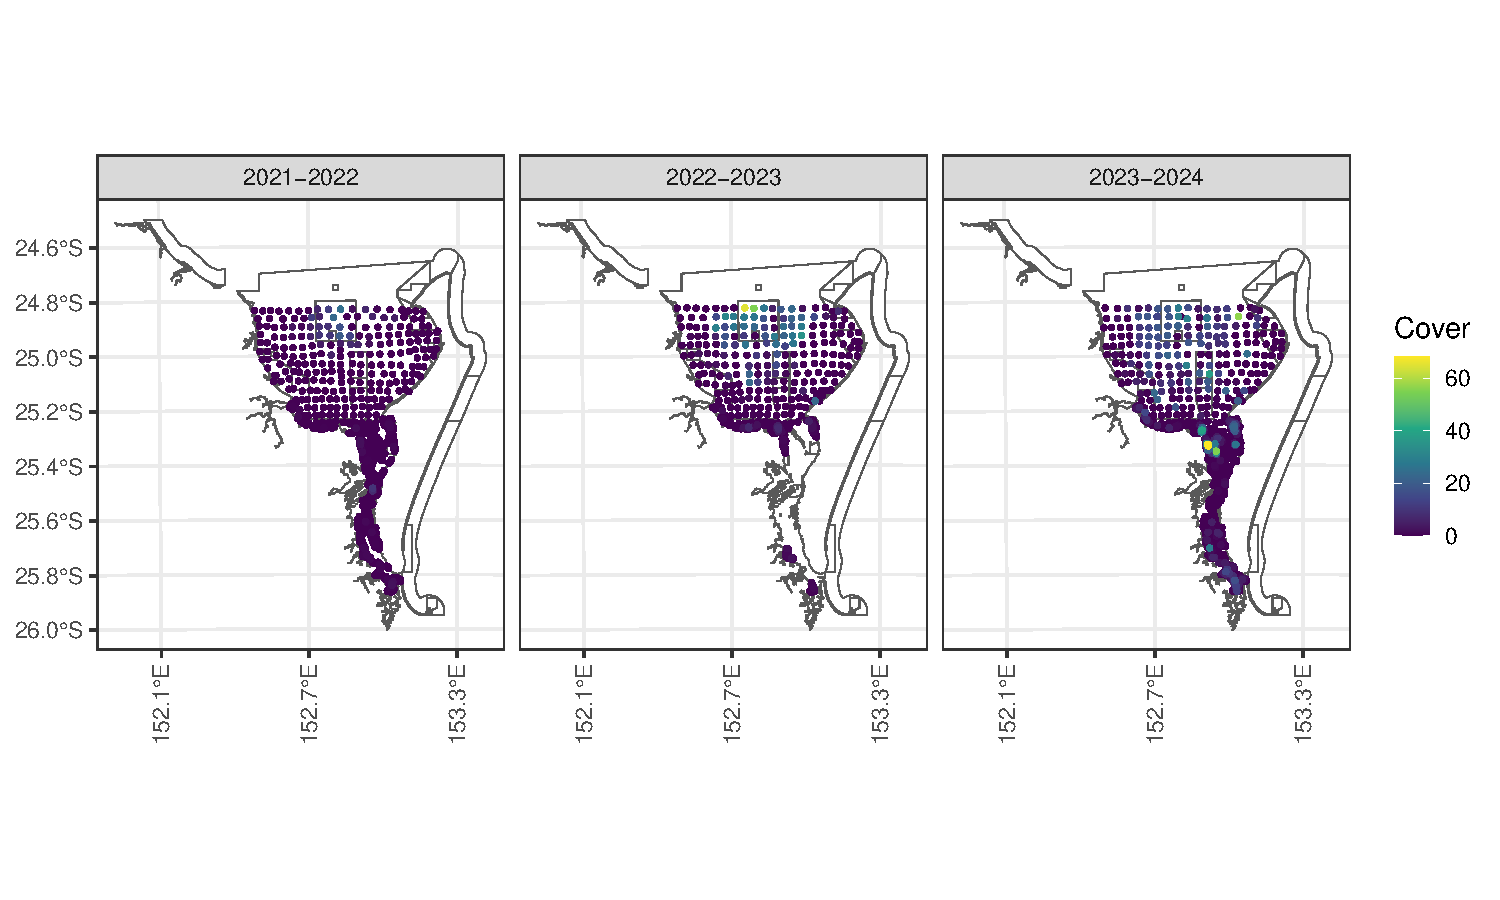
\includegraphics[keepaspectratio]{WBreport_files/figure-pdf/fig-cover_fy_wb-1.pdf}}

}

\caption{\label{fig-cover_fy_wb}Total seagrass cover in Wide Bay by
financial year.}

\end{figure}%

EcoFutures Consulting used eReefs data \citep{steven2019ereefs} to
generate a broad suite of ambient and flood-related turbidity, salinity,
and temperature variables at biologically and ecologically relevant
temporal windows (Table~\ref{tbl-wq_vars_wb}). Ambient water quality
variables were based on the mean, minimum, and maximum values for three
periods: 7, 30, and 90 days prior to sampling. Ambient variables were
also calculated representing the frequency of days water quality
thresholds were exceeded (above or below) and the maximum spell (i.e.,
duration) of days those thresholds were continuously exceeded during the
time periods. Similar water quality variables representing flood-event
conditions were also calculated for the two separate 30-day flood
periods.

\begin{table}

\caption{\label{tbl-wq_vars_wb}Wide Bay water quality variables
considered in the exploratory analyses, including the variable name and
measurement unit (in parentheses), the type of water-quality variable
(Ambient, Flood), the time period in days, statistic calculated, and the
threshold value used (if any).}

\centering{

\centering
\begin{tabular}{lllll}
  \toprule
Variable & Type & Period & Statistic & Threshold \\ 
  \midrule
Turbidity (NTU) & Ambient & 30, 7, 90 & Mean &  \\ 
  Turbidity (NTU) & Ambient & 30, 7, 90 & Frequency & $>$ 3 \\ 
  Turbidity (NTU) & Ambient & 30, 7, 90 & Frequency & $>$ 5 \\ 
  Turbidity (NTU) & Ambient & 30, 7, 90 & Frequency & $>$ 6 \\ 
  Salinity (PSU) & Ambient & 30, 7, 90 & Frequency & $<$ 20 \\ 
  Salinity (PSU) & Ambient & 30, 7, 90 & Frequency & $<$ 25 \\ 
  Salinity (PSU) & Ambient & 30, 7, 90 & Frequency & $<$ 30 \\ 
  Temperature (deg C) & Ambient & 30, 7, 90 & Mean &  \\ 
  Turbidity (NTU) & Flood & 30 & Mean &  \\ 
  Turbidity (NTU) & Flood & 30 & Max &  \\ 
  Turbidity (NTU) & Flood & 30 & Frequency & $>$ 3 \\ 
  Turbidity (NTU) & Flood & 30 & Frequency & $>$ 5 \\ 
  Turbidity (NTU) & Flood & 30 & Frequency & $>$ 6 \\ 
  Turbidity (NTU) & Flood & 30 & Duration & $>$ 3 \\ 
  Turbidity (NTU) & Flood & 30 & Duration & $>$ 5 \\ 
  Turbidity (NTU) & Flood & 30 & Duration & $>$ 6 \\ 
  Salinity (PSU) & Flood & 30 & Min &  \\ 
  Salinity (PSU) & Flood & 30 & Mean &  \\ 
  Salinity (PSU) & Flood & 30 & Frequency & $<$ 20 \\ 
  Salinity (PSU) & Flood & 30 & Frequency & $<$ 25 \\ 
  Salinity (PSU) & Flood & 30 & Frequency & $<$ 30 \\ 
  Salinity (PSU) & Flood & 30 & Duration & $<$ 20 \\ 
  Salinity (PSU) & Flood & 30 & Duration & $<$ 25 \\ 
  Salinity (PSU) & Flood & 30 & Duration & $<$ 30 \\ 
   \bottomrule
\end{tabular}

}

\end{table}%

Additional covariates were also provided by EcoFutures Consulting, which
are used to represent geographic features, depth, and algae cover, as
well as the years since the floods and the seagrass growing season.
These variables have the following structure:

\begin{itemize}
\tightlist
\item
  Sediment Type has six categorical levels: Sand, Sandy Mud, Muddy Sand,
  Mud, and Rock.
\item
  Tidal Range has three categorical levels: Shallow Subtidal,
  Intertidal, and Deep Subtidal.
\item
  Years Since Flood One is numeric ranging from 0.096 (May, 2022) to
  1.65 (November, 2023).
\item
  Years Since Flood Two is numeric ranging from 0 (May, 2022) to 1.65
  (November, 2023).
\item
  Algae Presence has two categorical levels: Algae present and algae not
  present.
\item
  Algae Cover is numeric ranging from 0 (no algae) to 100 (entire area
  covered in algae).
\item
  Growing Season has two categorical two levels: Growing (September -
  December) and Not Growing (January - August).
\item
  Zone class has six categorical levels: Central, East, Great Sandy
  Strait, Hervey Bay, Southern, and Southwest
  (Figure~\ref{fig-zone_class}).
\end{itemize}

\begin{figure}

\centering{

\pandocbounded{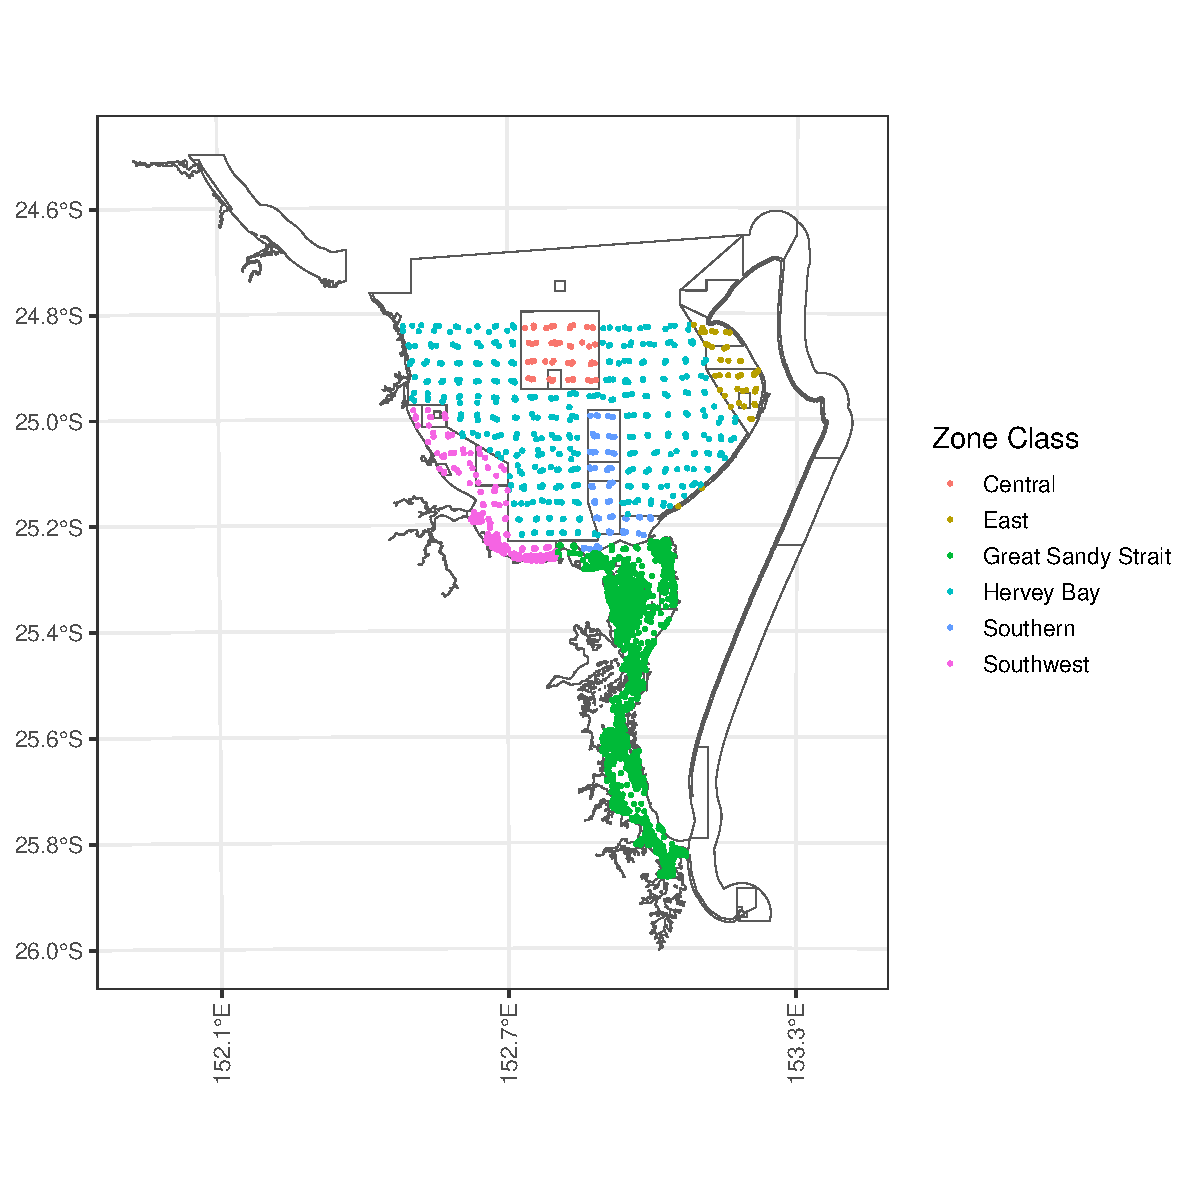
\includegraphics[keepaspectratio]{WBreport_files/figure-pdf/fig-zone_class-1.pdf}}

}

\caption{\label{fig-zone_class}Observations and their zone classes in
Wide Bay.}

\end{figure}%

\subsection{Exploratory Analyses}\label{exploratory-analyses}

Extensive exploratory analyses were undertaken to 1) understand the data
structure, 2) visualize spatial and temporal patterns in the data, 3)
identify outliers/errors, 4) examine correlations between potential
covariates and the seagrass cover, as well as multicollinearity among
covariates, 5) compare the fit of various models, and 6) evaluate model
assumptions.

Results revealed substantial collinearity among ambient and
flood-related water-quality variables, as expected given their nested
temporal windows and threshold values. We retained only one variable
from each correlated group. We prioritized including sediment type,
tidal range, turbidity, temperature, and time since floods, given a goal
was to study the extent to which these variables were related to
seagrass cover. While we had data for time since both floods, we removed
time since the second flood because these two variables were highly
collinear. The majority of the data were collected after the second
flood, in which case the variables are redundant. Rather than trying to
separate water quality effects from each of the two floods, we averaged
these effects across both floods to create a single turbidity metric
capturing flood-related impacts. We removed other variables showing no
meaningful association with seagrass cover or where the relationship
lacked biological plausibility. This included the salinity variables,
which had little variability and did not exhibit strong relationships
with seagrass cover. Geographic variables exhibited less collinearity
than water quality variables; however, we removed the algae variables
due to weak associations with seagrass cover after accounting for other
variables in the model. Growing season was excluded because a simple
monthly proxy inadequately captures seasonal seagrass growth dynamics.

The final set of potential covariates considered in the modelling
included mean turbidity in the 90 days prior to sampling, mean turbidity
during the flood event, mean temperature in the 90 days prior to
sampling, sediment type, tidal range, years since flood one, and EHMP
subzone.

\subsection{Statistical Modeling}\label{sec-wb_model}

We considered multiple modeling approaches in this study, which each
accounted for the data distribution, nonlinear relationships between
seagrass cover and covariates, and spatial dependence inherent in
biological data collected through space and time to different degrees
(Appendix 1). We used the full set of potential covariates to fit a
nonspatial linear model, spatial linear model (i.e., spatial model),
spatial beta regression model, spatial gamma regression model, and a
random forest model, comparing the model fit of each. We also considered
a spatial logistic regression model, treating seagrass as
presence/absence data; this model had similar drivers as the total
seagrass models and so we did not consider it further.

There were several reasons for fitting these initial models. The
nonspatial linear model provided a useful baseline to compare the
spatial linear model against, elucidating the impact of spatial
dependence on model fit. The spatial beta regression model is a
generalized linear model used to characterize proportion data ranging
between zero and one. To adhere to this restriction, total seagrass
cover was 1) scaled from a percentage to a proportion and 2) if exactly
zero or one, set to 0.01 or 0.99, respectively. The spatial gamma
regression model is a generalized linear model used to characterize
skewed positive data. To adhere to this restriction, a value of 0.01 was
added to seagrass cover observations that were equal to zero. Finally,
the random forest model provided a useful assessment of a machine
learning approach, which requires fewer distributional assumptions than
the aforementioned statistical approaches and more naturally describes
nonlinear relationships between variables (Appendix 1). We also
characterized random forest effects using partial dependence plots
\citep{greenwell2017pdp}, which isolate the marginal contribution of a
variable while holding other variables at their observed values.
Out-of-sample predictions were generated for the four statistical models
using leave-one-out cross validation, while out-of-bag validation was
used for the random forest model. These out-of-sample predictions were
then used to calculate the mean bias (MBias) and
root-mean-square-prediction error (RMSPE) for each model.

The results of this initial model comparison showed that the random
forest had the lowest RMSPE, followed by the spatial linear model,
generalized linear models, and the nonspatial linear model
(Table~\ref{tbl-wb_cv}). The nonspatial and spatial linear models also
had considerably lower mean bias values than the random forest model,
while the two generalized linear models produced unacceptably biased
predictions. Overall, all five approaches generally identified similar
relationships between seagrass cover and the covariates, in the
directions expected (when there were significant effects). There were
some minor differences in the effect of turbidity among the modeling
approaches, which we briefly note later. Random forest partial
dependence plots \citep{greenwell2017pdp} suggested that linear effects
of the model variables were generally reasonable. Given these results
and the ease of interpretability of the spatial linear model, we chose
to use a spatial linear modeling framework for the Wide Bay seagrass
cover model.

\begin{table}

\caption{\label{tbl-wb_cv}Wide Bay out of sample prediction metrics for
the various approaches. Mean bias (MBias) tended to be small relative to
root-mean-squared-prediction error (RMSPE). For LM, SPLM, SPGLM-Beta,
SPGLM-Gamma, leave-one-out cross validation was used. For RF, out of bag
validation was used.}

\centering{

\centering
\begin{tabular}{lrr}
  \toprule
Approach & MBias & RMSPE \\ 
  \midrule
Random Forest & -0.029 & 4.537 \\ 
  Spatial Linear Model & -0.003 & 4.700 \\ 
  Spatial GLM - Gamma & 1.177 & 5.116 \\ 
  Spatial GLM - Beta & -0.159 & 5.306 \\ 
  Linear Model & -0.000 & 5.452 \\ 
   \bottomrule
\end{tabular}

}

\end{table}%

\begin{figure}

\centering{

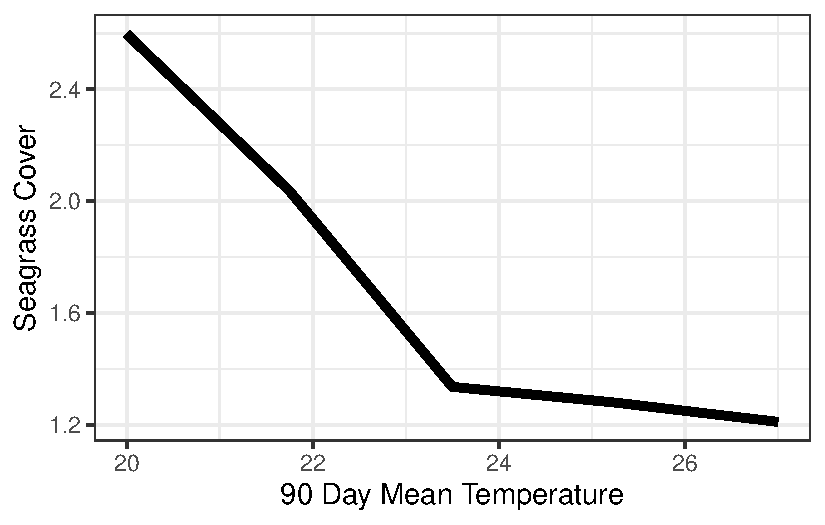
\includegraphics[width=0.5\linewidth,height=\textheight,keepaspectratio]{WBreport_files/figure-pdf/fig-rf_temp-1.pdf}

}

\caption{\label{fig-rf_temp}Random forest partial dependence for total
seagrass percent cover as a function of 90 day mean temperature.}

\end{figure}%

A suite of spatial linear models (Appendix 1, Equation~\ref{eq-splm1}),
with exponential spatial covariance functions and a random effect for
zone class, were fit using the \texttt{splm()} function in
\texttt{spmodel} \citet{dumelle2023spmodel}. Parameters were estimated
using restricted maximum likelihood. Parameters were estimated using
restricted maximum likelihood and models primarily compared model using
leave-one-out cross validation fit statistics; though AIC or BIC could
also be used if parameters were estimated using maximum likelihood. In
addition, the relationships between seagrass cover and covariates needed
to be plausible.

The final total seagrass cover model for Wide Bay included the following
covariates: tidal range, sediment type, 90-day mean temperature (prior
to sampling), 90 day turbidity (prior to sampling), and mean turbidity
during flood period one scaled by time since the flood squared
(Table~\ref{tbl-wb_tc_splm_vars}). Mean turbidity during flood period
one was scaled so that its effect decays with time since the flood.
Intuitively, this means that as the time since flood one increases, the
impact of turbidity during the flood event decreases. We also considered
scaling by time since flood one (not squared), which produced similar
results. This modeling approach is similar to the Moreton Bay modeling
approach \citep{dumelle2026moreton}, as similar research questions were
asked for each region.

\begin{table}

\caption{\label{tbl-wb_tc_splm_vars}Covariates in the final Wide Bay
seagrass cover model, their type (numeric or categorical), and if
categorical, the number of unique levels.}

\centering{

\centering
\begin{tabular}{lll}
  \toprule
Variable & Type & No. Levels \\ 
  \midrule
90 Day Temperature & Numeric & NA \\ 
  90 Day Turbidity & Numeric & NA \\ 
  Mean Flood Turbidity/Years Since Flood One\verb|^|2 & Numeric & NA \\ 
  Sediment Type & Categorical & 5 \\ 
  Tidal Range & Categorical & 3 \\ 
   \bottomrule
\end{tabular}

}

\end{table}%

\begin{table}

\caption{\label{tbl-wb-fixed}Fixed effects table of covariates in the
Wide Bay water quality and geographic model.}

\centering{

\centering
\begin{tabular}{lrrr}
  \toprule
Term & Estimate & z & p.value \\ 
  \midrule
Intercept (Mud/Deep Subtidal) & 14.405 & 5.111 & 0.000 \\ 
  Intertidal & 0.419 & 0.969 & 0.333 \\ 
  Shallow Subtidal & 1.652 & 1.955 & 0.051 \\ 
  Muddy Sand & -1.060 & -1.822 & 0.068 \\ 
  Rock & -1.264 & -1.282 & 0.200 \\ 
  Sand & -0.685 & -1.195 & 0.232 \\ 
  Sandy Mud & -1.492 & -2.700 & 0.007 \\ 
  90 Day Temperature & -0.502 & -7.411 & 0.000 \\ 
  90 Day Turbidity & 0.844 & 1.371 & 0.170 \\ 
  Mean Flood Turbidity/Years Since Flood One\verb|^|2 & -0.000 & -0.050 & 0.960 \\ 
   \bottomrule
\end{tabular}

}

\end{table}%

Table~\ref{tbl-wb-fixed} shows the fixed effects table from the fitted
model. The reference group is the muddy and deep subtidal group, and the
remaining sediment type and tidal range terms represent deviations from
these baselines. For the numeric variables, temperature had a small
\(p\)-value (\(p\)-value \(<\) 0.01) while the turbidity metrics had
large \(p\)-values (\(p\)-values \textgreater{} 0.1). While we can
assess the overall significance of the numeric variables
Table~\ref{tbl-wb-fixed}, we must perform an analysis of variance
(ANOVA) to assess the overall significance of variables with many
levels. Table~\ref{tbl-wb-covariates} shows these ANOVA results for the
sediment type and tidal range variables; sediment type had a small
\(p\)-value (\(p\)-value \(<\) 0.01) while tidal range had a larger
\(p\)-value (\(p\)-value \textgreater{} 0.1). Together, these results
indicate sediment type and temperature had significant effects on
seagrass cover, while there was not substantial evidence the other
variables did, at least in these data. Here are some relevant takeaways
from the model fit for the sediment type and temperature variables:

\begin{itemize}
\tightlist
\item
  Sediment Type: The estimated (marginal) average seagrass cover is
  largest in mud (4.3\%), followed by sand (3.6\%), muddy sand (3.2\%),
  rock (3.0\%), and sandy mud (2.8\%).
\item
  90 Day Temperature: A one-degree (C) increase in 90 day temperature is
  associated with a decrease in average total cover by 0.5\% points.
\end{itemize}

\begin{table}

\caption{\label{tbl-wb-covariates}ANOVA table of covariates for the
categorical variables in the Wide Bay water quality and geographic
model.}

\centering{

\centering
\begin{tabular}{lrrr}
  \toprule
Effects & df & Chi-sq & p.value \\ 
  \midrule
Sediment Type &    4 & 16.638 & 0.002 \\ 
  Tidal Range &    2 & 3.870 & 0.144 \\ 
   \bottomrule
\end{tabular}

}

\end{table}%

\begin{figure}

\centering{

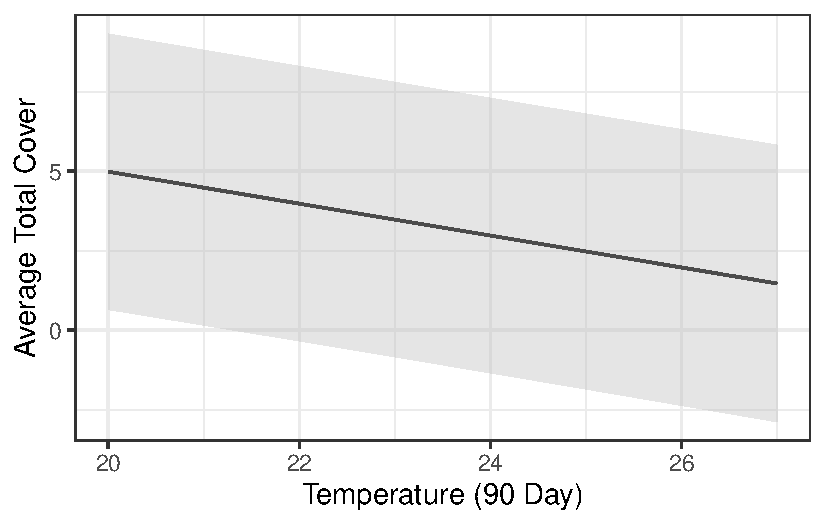
\includegraphics[width=0.5\linewidth,height=\textheight,keepaspectratio]{WBreport_files/figure-pdf/fig-wb_temp_90d-1.pdf}

}

\caption{\label{fig-wb_temp_90d}Average total cover as a function of 90
day mean temperature. Estimates (and confidence intervals) were
evaluated at the means of all other numeric variables, and for the
intertidal range and Sand sediment types.}

\end{figure}%

We examined model diagnostics to better understand the overall model
fit. First, we partitioned the model into different components of
variability (Table~\ref{tbl-wb_varcomp}) and found that 5.4\% is
attributable to the covariates (a quantity sometimes referred to as the
Pseudo R-squared), 54.2\% to the spatial random error, 5.8\% to the zone
class, and the remaining variability is independent random error.
Second, we examined the decay behaviour of spatial autocorrelation. The
estimated exponential spatial range (\(\phi\)) is 14757 meters, which
suggests two total cover observations are approximately (spatially)
uncorrelated at a distance of \(3\phi \approx 45\)km, or forty-five
kilometers. Third, we analyzed the standardized model residuals, which
have been decorrelated, to assess model assumptions and identify
influential observations that had a sizable impact on model fit.
Generally, the standardized residuals are centered around zero, though
there is a slight right skew suggesting some observed total cover values
are larger than expected (according to the model). Observations are
referred to as ``influential'' if they highly influence model fit.
Influence is often assessed using a Cook's distance threshold value of
one \citep{cook1982residuals}. No observations exceed this threshold.

\begin{table}

\caption{\label{tbl-wb_varcomp}Variance components in the Wide Bay
seagrass model.}

\centering{

\centering
\begin{tabular}{llr}
  \toprule
Variance Component & Percent (of Total Variability) & Parameter Value \\ 
  \midrule
Covariates & 5.4\% &  \\ 
  Spatial Effect & 54.2\% & 28.8 \\ 
  Independent Error & 34.6\% & 18.4 \\ 
  Zone Class & 5.8\% & 14757.0 \\ 
   \bottomrule
\end{tabular}

}

\end{table}%

All five modeling approaches found significant relationships between
sediment type and temperature. The nonspatial linear model and spatial
beta regression model found significant, negative relationships between
turbidity and total cover overall, while the random forest ranked
turbidity as important metrics. All but the spatial linear model and
random forest found significant relationships among tidal ranges, with
intertidal or deep subtidal having the lowest average total cover. For
the random forest, tidal range was the least important variable.

\subsection{Block Kriging}\label{block-kriging}

A tremendous benefit of using the spatial linear model is that block
Kriging \citep{ver2002sampling, cressie2006block} can be used to predict
the mean total seagrass cover bay-wide for any combination of covariates
and geographic regions, even if these variables were not directly used
in the model (see Appendix 1 for additional details). Block Kriging was
undertaken, by financial year, for zone class, Marine Park zone, tidal
range and for the whole of Wide Bay.

Figure~\ref{fig-bk_wb_class}, Figure~\ref{fig-bk_wb_zone}, and
Figure~\ref{fig-bk_wb_tidal} show that seagrass cover has generally
improved since 2021-2022 across all zone classes, conservation zones,
and tidal ranges. Although there were notable declines observed in
Marine National Park Zones between 2022-2023 and 2023-2024
(Figure~\ref{fig-bk_wb_zone}). When we examine recovery for the whole of
Wide Bay (Figure~\ref{fig-bk_wb_all}), the model suggests that seagrass
cover has improved since 2021-2022, but the same declines are observed
between 2022-2023 and 2023-2024.

\begin{figure}

\centering{

\pandocbounded{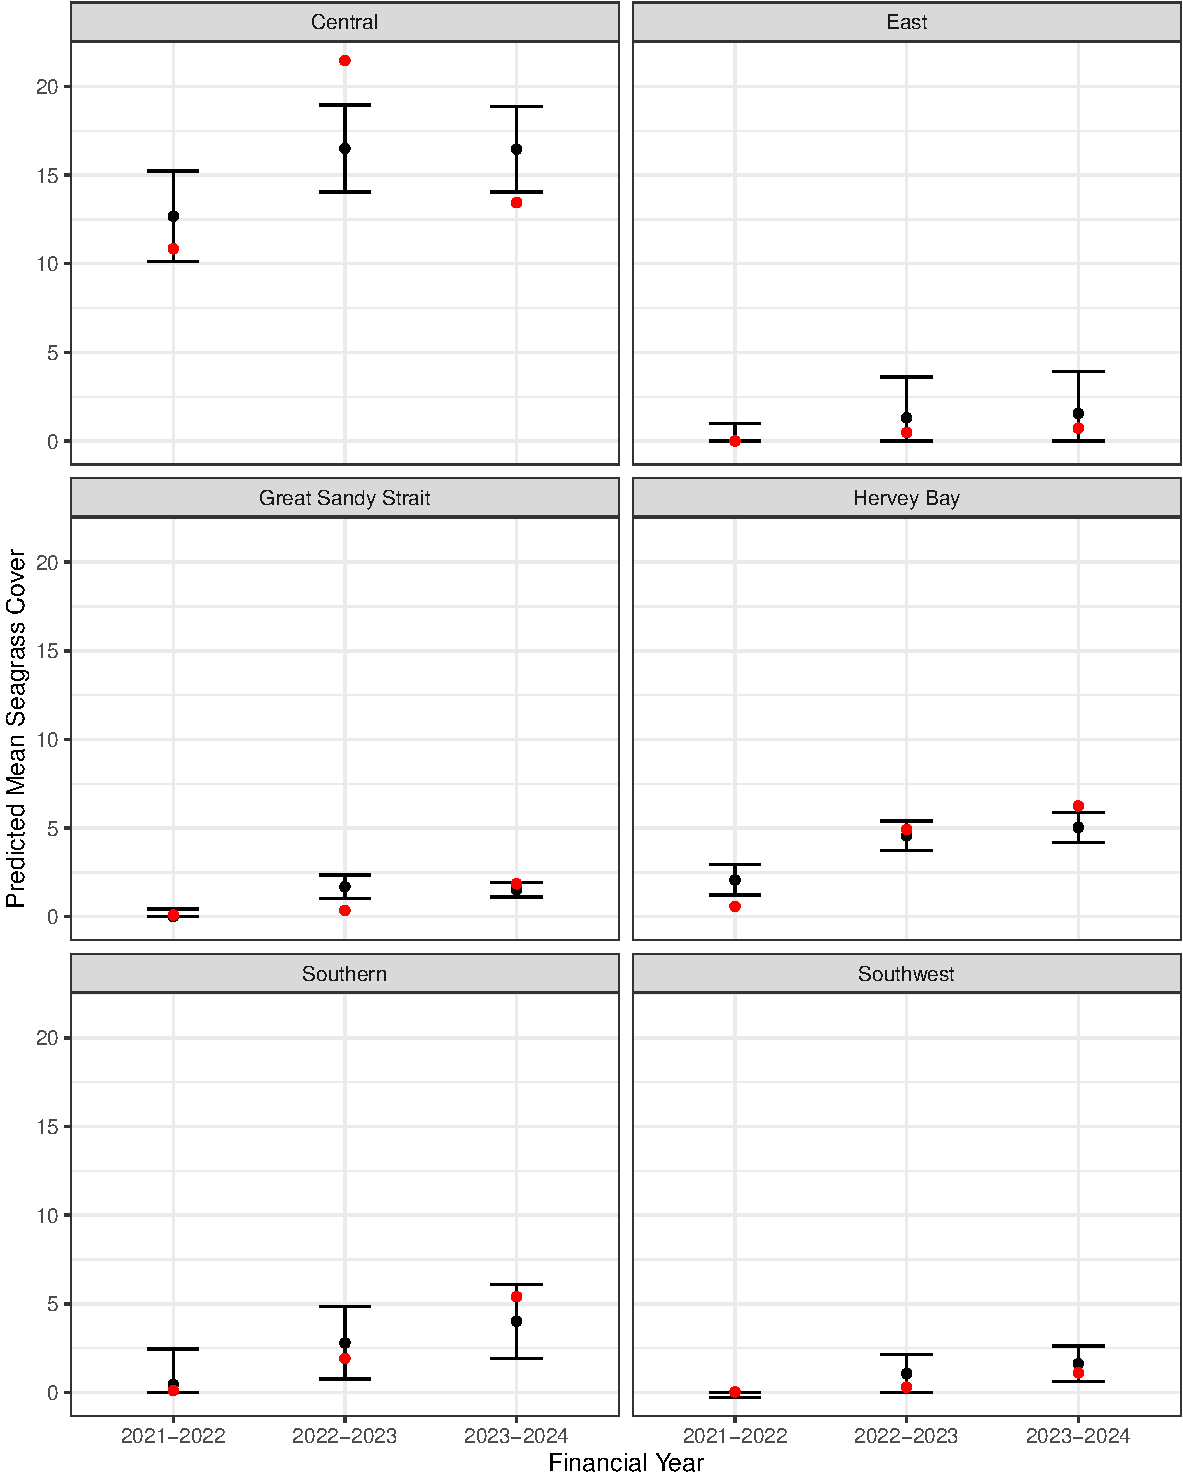
\includegraphics[keepaspectratio]{WBreport_files/figure-pdf/fig-bk_wb_class-1.pdf}}

}

\caption{\label{fig-bk_wb_class}Average seagrass cover predictions by
zone class. Red dots indicate the mean from the raw data. Black dots
indicate the predicted mean in the region alongside a prediction
interval.}

\end{figure}%

\begin{figure}

\centering{

\pandocbounded{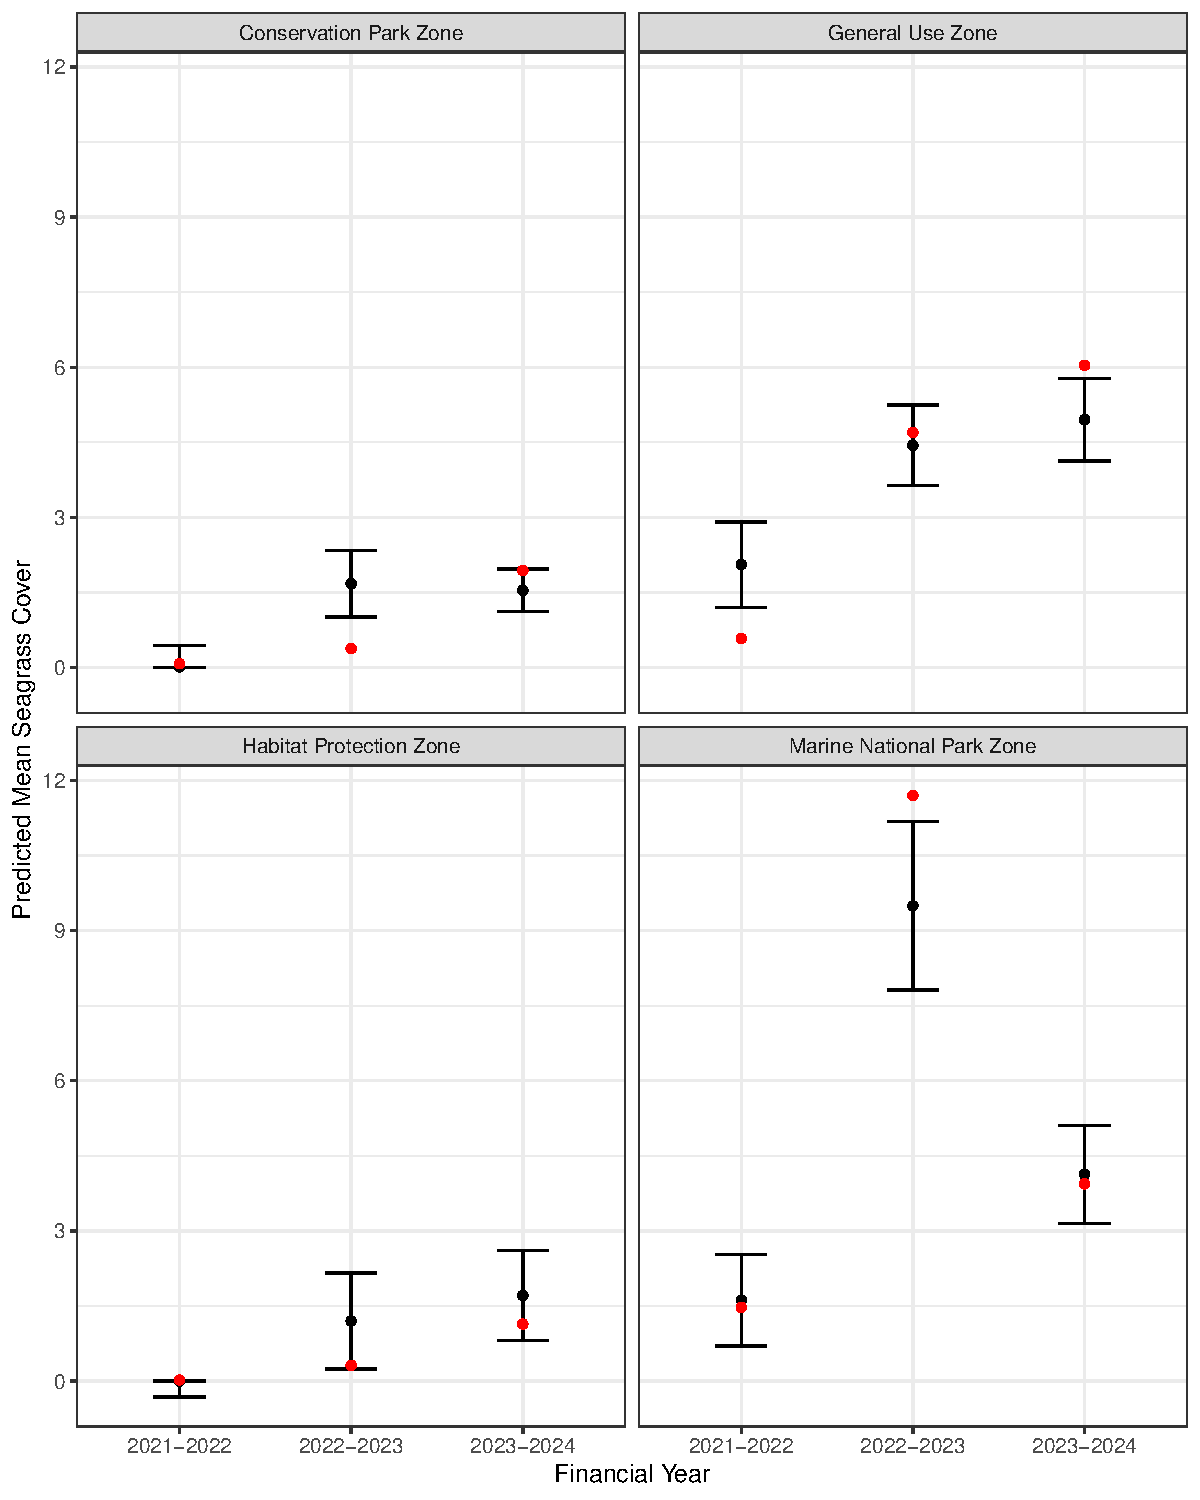
\includegraphics[keepaspectratio]{WBreport_files/figure-pdf/fig-bk_wb_zone-1.pdf}}

}

\caption{\label{fig-bk_wb_zone}Average seagrass cover predictions by
conservation zone. Red dots indicate the mean from the raw data. Black
dots indicate the predicted mean in the region alongside a prediction
interval.}

\end{figure}%

\begin{figure}

\centering{

\pandocbounded{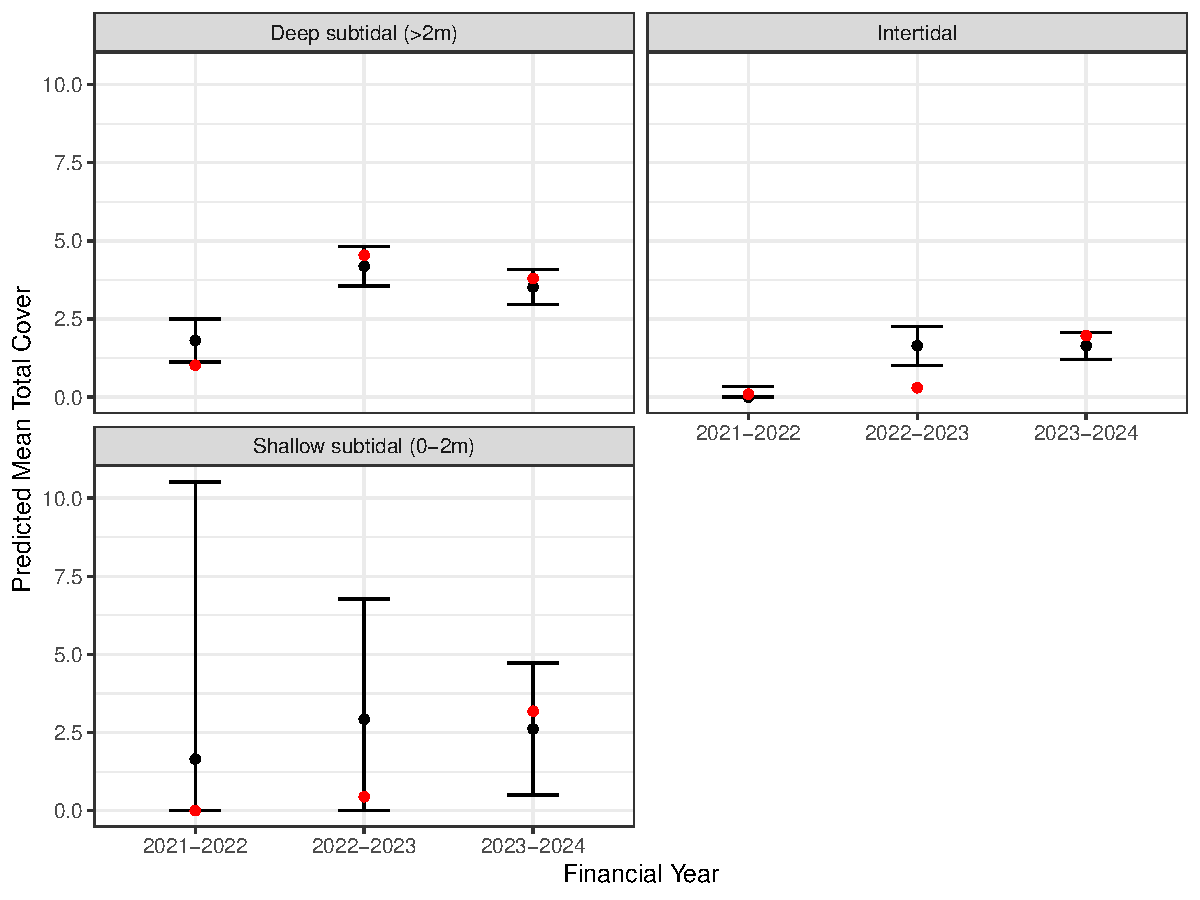
\includegraphics[keepaspectratio]{WBreport_files/figure-pdf/fig-bk_wb_tidal-1.pdf}}

}

\caption{\label{fig-bk_wb_tidal}Average seagrass cover predictions by
tidal range. Red dots indicate the mean from the raw data. Black dots
indicate the predicted mean in the region alongside a prediction
interval.}

\end{figure}%

\begin{figure}

\centering{

\pandocbounded{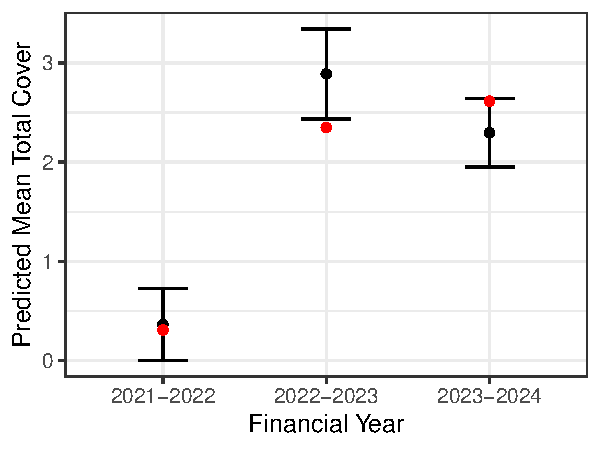
\includegraphics[keepaspectratio]{WBreport_files/figure-pdf/fig-bk_wb_all-1.pdf}}

}

\caption{\label{fig-bk_wb_all}Average seagrass cover predictions in Wide
Bay. Red dots indicate the mean from the raw data. Black dots indicate
the predicted mean in the region alongside a prediction interval.}

\end{figure}%

\clearpage

\section{Resilience Modeling}\label{sec-wb_resilience}

The seagrass cover model quantifies bay-wide effects of influential
drivers on seagrass cover and enables assessment of recovery
trajectories at management-relevant scales. However, it does not
quantify site-specific resilience. \citet{gilby2023drivers} propose
identifying hotspots (i.e., brightspots, sites performing better than
expected) and coldspots (sites performing worse than expected) based on
model residuals exceeding confidence interval bounds. They argue that
hotspots and coldspots offer significant utility for understanding
drivers of site-specific resilience and informing management decisions.
\citet{gilby2023drivers} primarily focused on specific hotspots, linking
environmental variables to those sites. We build on that work by using
the seagrass model residuals as a proxy for site-specific resilience,
and then characterizing the most important drivers of that resilience.

\subsection{Data}\label{data-1}

We used the raw seagrass model residuals (Figure~\ref{fig-resid_fy_wb})
as a the response variable in a second spatial linear model used to
study site-specific resilience in Wide Bay. Model covariates included
variables describing seagrass richness and dominant species, and
bathymetry, as well as distance to the nearest coral, seagrass,
mangrove, or gastropod habitat, and the total area of coral, seagrass,
mangrove, or gastropod habitat within 500 m of the observation point
(Table~\ref{tbl-res_vars_wb}). The Zone class was again included as a
random effect. Because we were interested in hypothesis testing rather
than parsimony, we included all potential covariates as fixed effects in
the model. Potential covariates have the following structure:

\begin{itemize}
\tightlist
\item
  Coral Habitat Total Area is numeric from 0 to 367,906 meters squared
  (msq).
\item
  Seagrass Habitat Total Area is numeric from 0 to 773,161 msq.
\item
  Mangrove Habitat Total Area is numeric from 0 to 241,057 msq.
\item
  Distance to Coral Habitat is numeric from 0 to 30,563 m.
\item
  Distance to Seagrass Habitat is numeric from 0 to 7,049 m.
\item
  Distance to Mangrove Habitat is numeric from 0 to 38,867 m.
\item
  Distance to Gastropod Habitat is numeric from 0 to 121,609 m.
\item
  Habitat Count is numeric (integer) from 0 to 3 unique habitats (coral,
  seagrass, mangrove).
\item
  Species Richness is numeric (integer) from 0 to 4 unique species
  (possible species: ``Absent'', ``HD'', ``HO'', ``HS'', and ``ZMHU'').
\item
  Dominant Species represents the dominant seagrass species and has five
  levels: ``Absent'', ``HD'', ``HO'', ``HS'', and ``ZMHU''.
\item
  Bathymetry Mean Depth is the GBR mean depth within 500 m of the
  seagrass observation point, excluding terrestrial areas, and is
  numeric from -30.58 m to 0.25 m.
\item
  Bathymetry Mean Curvature is the GRB mean curvature within 500 m of
  the seagrass observation point, excluding terrestrial areas, and is
  numeric from -0.001 to 0.001.
\item
  Bathymetry Mean Slope is the GBR mean slope within 500 m of the
  seagrass observation point, excluding terrestrial areas, and is
  numeric from 0.004 degrees to 3.93 degrees.
\item
  Zone class has six categorical levels: Central, East, Great Sandy
  Strait, Hervey Bay, Southern, and Southwest.
\end{itemize}

We expected there to be nonlinear relationships between the response and
covariates and we accounted for them using B-spline basis functions
\citep{deboor1978practical, eilers1996flexible}. The degree of these
functions was informed by partial dependence plots derived from a random
forest model fitted to the seagrass model residuals
(Table~\ref{tbl-res_vars_wb}). We did not use the ``Gastropod Habitat
Total Area'' variable because there was no gastropod habitat overlap in
the Wide Bay data.

\begin{figure}

\centering{

\pandocbounded{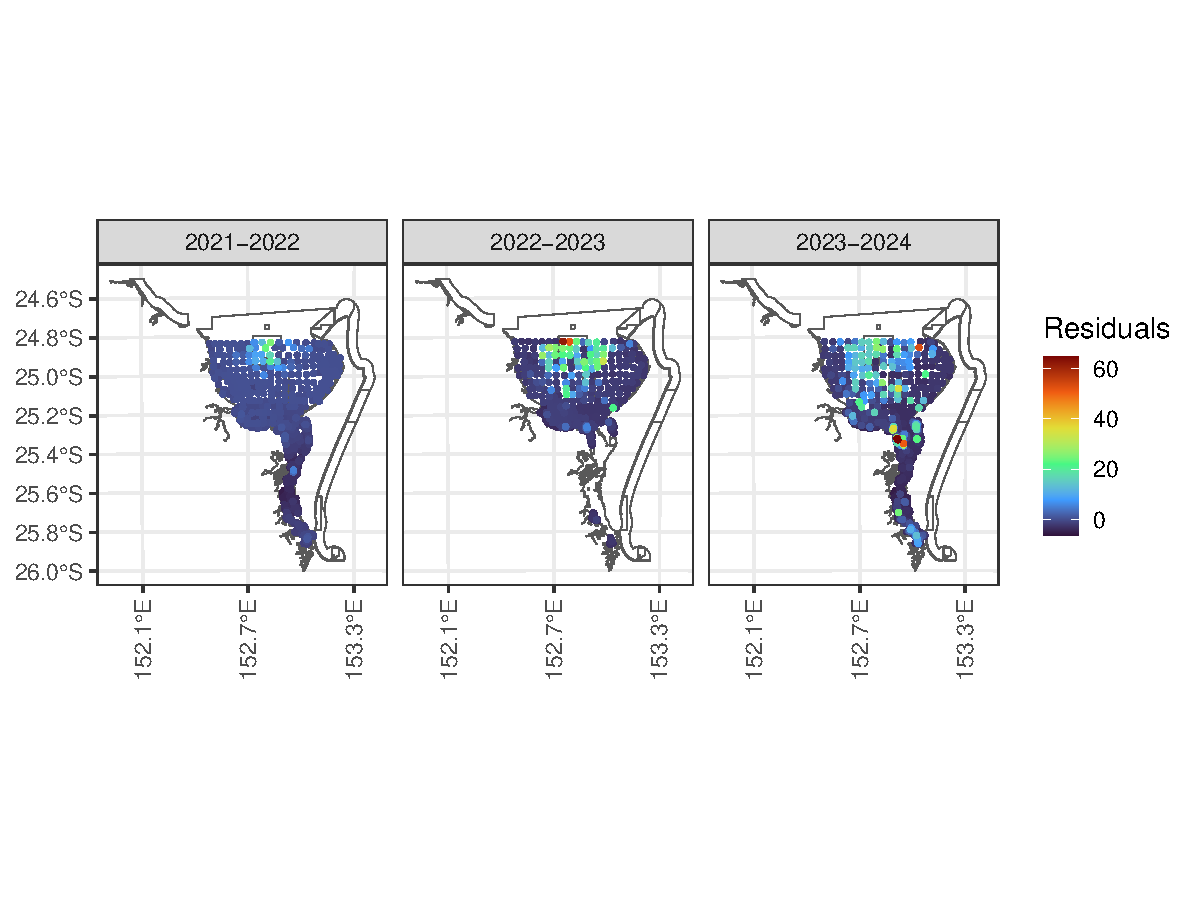
\includegraphics[keepaspectratio]{WBreport_files/figure-pdf/fig-resid_fy_wb-1.pdf}}

}

\caption{\label{fig-resid_fy_wb}Seagrass model residuals for resilience
analysis in Wide Bay, by financial year.}

\end{figure}%

\begin{table}

\caption{\label{tbl-res_vars_wb}Covariates included in the resilience
model, including whether they were a fixed or random effect, and the
nonlinearity degree of the B-splines basis function.}

\centering{

\centering
\begin{tabular}{lll}
  \toprule
Variable & Effect & Degree \\ 
  \midrule
Coral Habitat Total Area & Fixed & 2 \\ 
  Seagrass Habitat Total Area & Fixed & 2 \\ 
  Mangrove Habitat Total Area & Fixed & 2 \\ 
  Distance to Coral Habitat & Fixed & 2 \\ 
  Distance to Seagrass Habitat & Fixed & 2 \\ 
  Distance to Mangrove Habitat & Fixed & 2 \\ 
  Distance to Gastropod Habitat & Fixed & 2 \\ 
  Species Richness & Fixed & 1 \\ 
  Habitat Count & Fixed & 2 \\ 
  Dominant Species & Fixed & NA \\ 
  Bathymetry Mean Depth & Fixed & 2 \\ 
  Bathymetry Mean Curvature & Fixed & 2 \\ 
  Bathymetry Mean Slope & Fixed & 2 \\ 
  Zone Class & Random & NA \\ 
   \bottomrule
\end{tabular}

}

\end{table}%

\subsection{Statistical Modeling}\label{statistical-modeling}

\begin{table}

\caption{\label{tbl-wb-res-fixed}Fixed effects table of covariates in
the Wide Bay resilience model.}

\centering{

\centering
\begin{tabular}{lrrr}
  \toprule
Term & Estimate & z & p.value \\ 
  \midrule
Intercept (Absent) & -1.278 & -0.416 & 0.677 \\ 
  HD & -1.329 & -1.936 & 0.053 \\ 
  HO & -1.659 & -2.160 & 0.031 \\ 
  HS & 1.427 & 1.893 & 0.058 \\ 
  ZMHU & -2.274 & -4.833 & 0.000 \\ 
  Species Richness & 5.245 & 15.449 & 0.000 \\ 
  Coral Area Deg1 & 0.757 & 0.305 & 0.760 \\ 
  Coral Area Deg2 & -0.167 & -0.057 & 0.954 \\ 
  Seagrass Area Deg1 & -0.745 & -0.967 & 0.334 \\ 
  Seagrass Area Deg2 & 0.408 & 0.774 & 0.439 \\ 
  Mangrove Area Deg1 & 0.973 & 0.498 & 0.619 \\ 
  Mangrove Area Deg2 & -2.951 & -1.058 & 0.290 \\ 
  Habitat Count Deg1 & -0.146 & -0.166 & 0.868 \\ 
  Habitat Count Deg2 & -0.143 & -0.169 & 0.866 \\ 
  Coral Distance Deg1 & -5.142 & -4.164 & 0.000 \\ 
  Coral Distance Deg2 & 11.490 & 7.074 & 0.000 \\ 
  Seagrass Distance Deg1 & -0.996 & -0.485 & 0.628 \\ 
  Seagrass Distance Deg2 & -0.922 & -0.440 & 0.660 \\ 
  Mangrove Distance Deg1 & 1.532 & 0.885 & 0.376 \\ 
  Mangrove Distance Deg2 & -2.174 & -1.279 & 0.201 \\ 
  Gastropod Distance Deg1 & -1.897 & -0.919 & 0.358 \\ 
  Gastropod Distance Deg2 & -2.619 & -1.747 & 0.081 \\ 
  Bathymetry Mean Depth Deg1 & 1.630 & 0.669 & 0.503 \\ 
  Bathymetry Mean Depth Deg2 & 1.192 & 0.621 & 0.535 \\ 
  Bathymetry Mean Slope Deg1 & -1.434 & -0.894 & 0.371 \\ 
  Bathymetry Mean Slope Deg2 & 0.920 & 0.264 & 0.792 \\ 
  Bathymetry Mean Curvature Deg1 & 0.465 & 0.169 & 0.866 \\ 
  Bathymetry Mean Curvature Deg2 & -0.014 & -0.007 & 0.994 \\ 
   \bottomrule
\end{tabular}

}

\end{table}%

Table~\ref{tbl-wb-res-fixed} shows the fixed effects table from the
fitted model. The reference group is the absent dominant species, and
the remaining dominant species terms represent deviations from this
baseline. Species richness, the only numeric variable with a single
level, had a large test statistic and small \(p\)-value (\(p\)-value
\(<\) 0.01). The other numeric variables were modeled using a B-spline
basis of degree two to capture nonlinearities. While we can assess the
overall significance of species richness in
Table~\ref{tbl-wb-res-fixed}, we must perform an analysis of variance
(ANOVA) to assess the overall significance the remaining variables with
multiple terms. Table~\ref{tbl-wb-res-anova} shows these ANOVA results.

\begin{table}

\caption{\label{tbl-wb-res-anova}ANOVA table of covariates in the Wide
Bay resilience model.}

\centering{

\centering
\begin{tabular}{lrrr}
  \toprule
Effects & df & Chi-sq & p.value \\ 
  \midrule
Dominant Species &    4 & 68.011 & 0.000 \\ 
  Distance to Coral Habitat &    2 & 51.788 & 0.000 \\ 
  Distance to Gastropod Habitat &    2 & 3.089 & 0.213 \\ 
  Distance to Mangrove Habitat &    2 & 2.866 & 0.239 \\ 
  Seagrass Habitat Total Area &    2 & 2.752 & 0.253 \\ 
  Mangrove Habitat Total Area &    2 & 1.163 & 0.559 \\ 
  Bathymetry Mean Slope &    2 & 0.810 & 0.667 \\ 
  Distance to Seagrass Habitat &    2 & 0.536 & 0.765 \\ 
  Bathymetry Mean Depth &    2 & 0.466 & 0.792 \\ 
  Bathymetry Mean Curvature &    2 & 0.119 & 0.942 \\ 
  Coral Habitat Total Area &    2 & 0.096 & 0.953 \\ 
  Habitat Count &    2 & 0.059 & 0.971 \\ 
   \bottomrule
\end{tabular}

}

\end{table}%

We found strong evidence (\(p\)-value \textless{} 0.001) that species
richness, dominant species, and distance to coral habitat are associated
with resilience:

\begin{itemize}
\tightlist
\item
  Species Richness: An increase of species richness by one species was
  associated with an average increase in resilience by approximately
  five points (Figure~\ref{fig-wb_res_rich_coral}).
\item
  Dominant Species: HS are the most resilient, followed by HD, HO, and
  ZMHU.
\item
  Distance to Nearest Coral Habitat: From 0 to around 10000 m, there is
  a decreasing trend with resilience (i.e., increasing distance
  decreases resilience). Upwards of 10000 m, there is an increasing
  trend with resilience (i.e., increasing distance increases
  resilience).
\end{itemize}

We found little evidence (\(p\)-value \textgreater{} 0.1) the remaining
variables were associated with resilience (after controlling for other
modeled variables).

\begin{figure}

\centering{

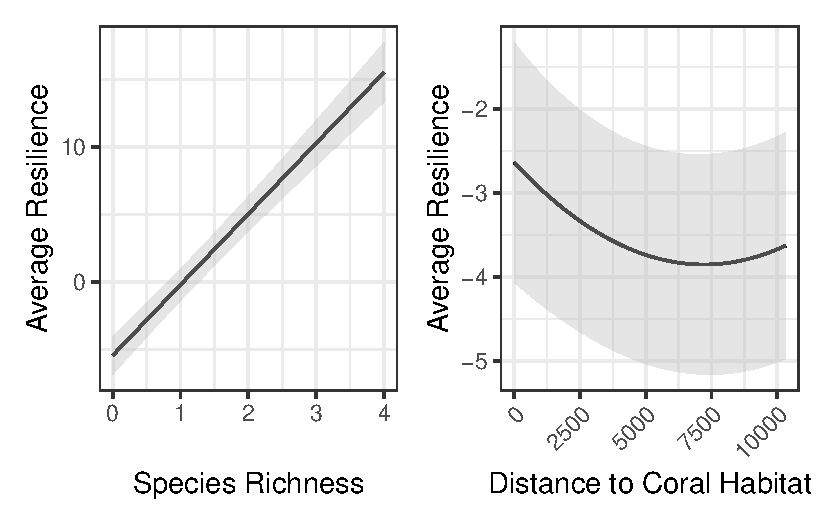
\includegraphics[width=0.8\linewidth,height=\textheight,keepaspectratio]{WBreport_files/figure-pdf/fig-wb_res_rich_coral-1.pdf}

}

\caption{\label{fig-wb_res_rich_coral}Average species richness (left)
and distance to coral habitat (right, for distances less than 10000 m)
effects on resilience. Estimates (and confidence intervals) were
evaluated at the means of all other numeric variables and for the ZMHU
species in the Central zone.}

\end{figure}%

As mentioned previously, we also fit a random forest model to the
seagrass model residuals. There were similarities and differences
between the spatial linear model and random forest. Notably, for the
random forest:

\begin{itemize}
\tightlist
\item
  Species richness was most important, with a general increasing trend
  in resilience with richness.
\item
  Distance to mangrove habitat was second-most important, with a general
  increasing trend in resilience with distance from mangroves.
\item
  Dominant species was third-most important, with HS being the most
  resilient followed by HO, ZMHU, and HD.
\item
  Bathymetry mean depth was fourth-most important, with a general
  increasing trend in resilience with depth.
\item
  Distance to gastropod habitat was fifth-most important, with a general
  decreasing trend in resilience with distance.
\item
  Distance to coral habitat was sixth-most important, with a similar
  quadratic trend (Figure~\ref{fig-rf_coral}) as in the spatial linear
  model.
\item
  Seagrass area was seventh-most important, with a general increasing
  trend in resilience with area.
\item
  The remaining variables (seagrass area, bathymetry slope, bathymetry
  curvature, zone class, seagrass distance, habitat count, mangrove
  area, and coral area) had notable drop offs in performance.
\end{itemize}

The consistency between the two resilience models' variable importance
rankings for species richness, dominant species, bathymetry mean depth,
and distance to both gastropod and coral habitats reinforces the spatial
linear model's identification of the most important drivers of
resilience. However, the random forest identifies distance to mangrove
habitat as the second most important variable, which is a questionable
finding given the direction of the relationship. This counterintuitive
result is likely a spurious correlation or an artifact of the random
forest model's inability to account for spatial dependence in the data,
which can affect variable importance measures \citep{fox2020comparing}.

\begin{figure}

\centering{

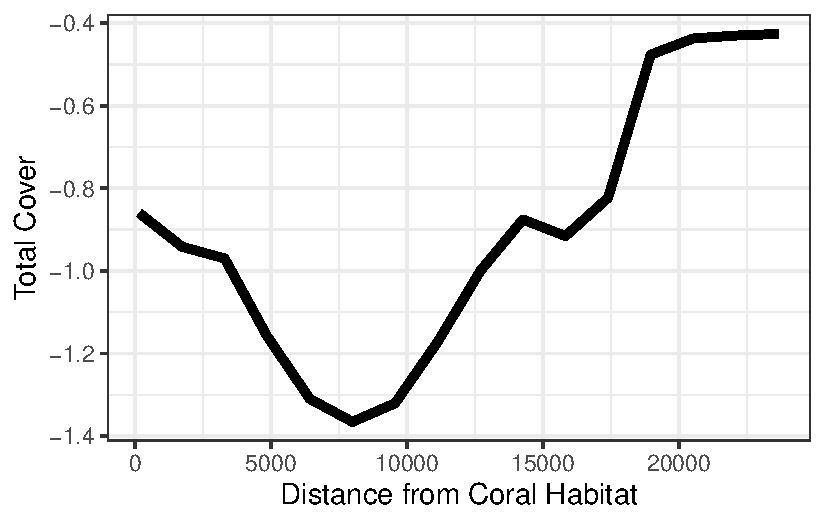
\includegraphics[width=0.5\linewidth,height=\textheight,keepaspectratio]{WBreport_files/figure-pdf/fig-rf_coral-1.pdf}

}

\caption{\label{fig-rf_coral}Random forest partial dependence for total
cover as a function of distance to coral habitat (for distances less
than 10000 m).}

\end{figure}%

\section{Limitations}\label{limitations}

While the spatial linear model was useful for characterizing broad
patterns in seagrass cover related to tidal range, sediment type,
temperature, and turbidity and site-specific patterns capturing
resilience, all while accounting for spatial dependence, there are some
limitations. First and foremost, seagrass cover data were not available
in the years prior to the first flood. Without a baseline, it is
impossible to quantify whether seagrass cover has recovered to pre-flood
levels. Second, the Wide Bay data are heavily skewed, with over 77\% of
observations containing no seagrass. This extreme skew compromised model
fit across all the approaches we explored. We selected the spatial
linear model because it naturally describes spatial dependence, offers
interpretability, and enables block Kriging predictions. However, the
model assumptions are less likely to hold given the sparse nonzero
observations, which undermines the reliability of model inferences.
Third, the eReefs water quality covariates are based on modeled data
that are not directly observed in the field, potentially propagating
modeling error. Fourth, there are many correlated water-quality
variables, making it difficult (for any model) to isolate the effects of
each component of water quality. Fifth, the lack of a covariate
describing mean salinity in the 90 days prior to sampling makes it
challenging to directly study the effect of mean salinity during the
flood period. Sixth, covariates representing local-scale drivers of
seagrass cover (e.g., light attenuation, biological interactions, etc.)
were not available, which might explain some additional variability in
the response through space and time. Finally, the location of sample
sites was not generated randomly and could be subject to conscious or
unconscious selection bias.

\section{Revisiting the Research
Questions}\label{revisiting-the-research-questions}

\textbf{Research Question 1}: Can we identify water quality covariates
that act as triggers for seagrass cover management responses? Are these
triggers different based on whether they result from a specific event
(e.g., flood) or are ambient?

We identified temperature as the primary water quality variable in the
seagrass cover model, with a one-degree increase in 90-day mean
temperature associated with a 0.5 percentage point decrease in cover.
This ambient temperature signal was statistically significant and
ecologically interpretable, as elevated temperatures may compound the
effects of other stressors on seagrass. In contrast, neither ambient
turbidity nor flood turbidity showed strong statistical evidence of
association with total cover after accounting for other variables. This
could result in part due to the absence of pre-flood baseline data,
which made it difficult to isolate the contribution of flood-driven
turbidity from background conditions. It could also be in part due to
the challenges associated with analyzing highly skewed data with many
zeros. Across tidal ranges, estimated average total cover was modest
throughout, and sediment type was a significant predictor, whereby muddy
substrates supported slightly higher average seagrass cover than sand,
sandy mud, or rock.

\textbf{Research Question 2}: Did seagrass cover improve after the flood
event(s)? If so, how and where?

Total seagrass cover has generally improved throughout Wide Bay between
financial years 2021-2022 and 2023-2024, suggesting the system may be
recovering from the floods. This improvement was seen across zone
classes, conservation zone types, tidal ranges, and bay-wide. However, a
decline in cover was observed in the Marine National Park Zone between
2022-2023 and 2023-2024 and this likely contributes to the slight
decline observed for Wide Bay as a whole in the same years. These
findings should be interpreted with care. The absence of pre-flood
baseline data means it is impossible to assess whether the observed
cover levels represent recovery relative to a pre-disturbance state or
simply reflect the current trajectory of the ecosystem.

\textbf{Research Question 3}: Can we identify site-specific resilience
indicators, which describe where recovery is likely to be enhanced or
impeded? What factors contribute to seagrass resilience?

We identified several site-specific indicators of seagrass resilience in
Wide Bay. Species richness and dominant species were the strongest
indicators of resilience, with each additional species associated with
an average increase in resilience of approximately five points. Sites
dominated by HS tend to be most resilient, followed by HD, HO, and ZMHU.
Distance to coral habitat was also a strong resilience indicator,
exhibiting a nonlinear pattern. Resilience declined with increasing
distance from coral up to approximately 10000 m, then increased beyond
that threshold, a pattern consistent with coral and seagrass occupying
different but adjacent positions along Wide Bay's water quality and
substrate gradient. These findings were broadly corroborated by the
random forest, which ranked species richness as the most important
predictor, dominant species, distance to mangrove habitat, bathymetry
mean depth, distance to gastropod habitat, distance to coral habitat,
and seagrass area. Together, these results suggest that management
actions protecting structurally diverse, species-rich meadows are likely
to be most effective at improving resilience, while sites with low
species richness (or no seagrass) may require more active intervention
to support recovery.

\section{Summary}\label{summary}

We applied a rigorous, spatially explicit statistical framework to
characterize the drivers, recovery, and resilience of seagrass cover in
Wide Bay across a three-year monitoring period that included the two
separate Wide Bay flood events. The analytical approach taken here is
well-suited to the structure and scale of the data, and the findings
have direct implications for adaptive management of the bay's seagrass
ecosystem.

The use of spatial linear models as the primary analytical framework is
well-justified from both statistical and ecological perspectives. Total
percent seagrass cover observations collected across the bay are
inherently spatially structured, as nearby sites share similar
environmental conditions, water quality and disturbance histories, as
well as ecological communities. Models that ignore this dependence may
well provide misleading results and inference. By explicitly modeling
spatial dependence via a spatial covariance function, the analyses
presented here produce more reliable estimates of covariate effects and
more honest characterizations of uncertainty than a conventional
non-spatial model provides. These models are typically also more
interpretable and characterize uncertainty more effectively than machine
learning models. The inclusion of zone class as a random effect further
accounts for structured variation among management-relevant regions of
the bay, ensuring that covariate estimates reflect within-zone patterns
rather than being confounded by between-zone differences in baseline
cover. The block Kriging helps understand bay-wide trends and can
immediately characterize bay-wide predictions on the original total
seagrass cover scale (0-100), rather than a transformed scale required
for generalized linear models; providing a flexible framework for
scenario modeling under future flood conditions and climate scenarios.

The use of a two-stage modeling framework -- first modeling total
seagrass cover as a function of water quality and geographic drivers,
then modeling the seagrass model residuals as a function of site-level
resilience covariates -- is a structured approach to separating bay-wide
environmental patterns from site-specific ecological resilience
capacity. This builds directly on the framework proposed by
\citet{gilby2023drivers} to help understand drivers of average
resilience and provide useful insight needed to inform broader
conservation strategies. The robustness of the findings is further
supported by the general consistency of results across multiple modeling
approaches (e.g., spatial beta regression model, random forest, etc.),
which provides evidence that the relationships identified are genuine
rather than resulting solely from specific modeling frameworks.

Overall, the results described in this report provide a quantitative,
spatially structured foundation for adaptive decision making. Together,
the identification of important water quality and geographic variables,
bay-wide predictions via block Kriging, and the characterization of
site-level resilience indicators provide data-driven evidence that can
inform temporally targeted, context-specific interventions throughout
the bay.

\clearpage

\section*{References}\label{references}
\addcontentsline{toc}{section}{References}

\renewcommand{\bibsection}{}
\bibliography{references.bib}

\section{Acknowledgements}\label{acknowledgements}

The eReefs datasets (model simulations, satellite or in-situ
observations) and software were produced as part of the eReefs project
(ereefs.org.au), which is a collaboration between Australia's national
science agency CSIRO, the Australian Institute of Marine Science (AIMS)
and the Queensland Government, with observations obtained through the
Integrated Marine Observing System (IMOS) and the Great Barrier Reef
Marine Park Authority (GBRMPA). eReefs is funded by the Australian
Government's Reef Trust.

\clearpage

\section*{Appendix 1. Spatial Linear Models and Random Forest
Models}\label{appendix-1.-spatial-linear-models-and-random-forest-models}
\addcontentsline{toc}{section}{Appendix 1. Spatial Linear Models and
Random Forest Models}

The spatially explicit statistical models (i.e., spatial models) we used
to answer these research questions are related to commonly used linear
and generalized linear models but incorporate \emph{spatial dependence}.
Spatial dependence measures how similar two sites are based on their
distance. Formally, we can build spatial dependence directly into
spatial models by leveraging Tobler's First Law of Geography
\citep{tobler1970computer}, which states succinctly that ``nearby sites
tend to be more similar than distant sites''. Not only is this intuitive
from a ``first principles'' perspective, but spatial models also provide
many advantages for modeling spatial data compared to models that assume
independence among observations (i.e., nonspatial models). First,
nonspatial models tend to underestimate uncertainty, yielding covariate
standard errors and p-values for covariates that are too small and
corresponding confidence intervals that are too narrow. Second, spatial
models improve prediction at unsampled locations by borrowing strength
from nearby observations, yielding more precise predictions and
corresponding standard errors that vary by location. Third, spatial
models decompose model error into separate spatial and nonspatial
components, informing residual and resilience structure in ways that
nonspatial models cannot. Fourth, spatial models can provide
ecologically meaningful insight into the spatial dependence structure of
the process, informing relationships among measured and unmeasured
variables as well as future sampling plans. \citet{zimmerman2024spatial}
provide a thorough review of spatial models for ecological and
environmental data, providing more detail and justification for the
claims made above.

Spatial models also offer many benefits over commonly used machine
learning algorithms like random forests
\citep{breiman2001random, cutler2007random, james2017introduction, kuhn2022tidy}.
First, traditional machine learning algorithms do not incorporate
spatial dependence and, by consequence, often perform worse than spatial
models at characterizing important covariates and predicting at
unobserved locations \citep{fox2020comparing}. Second, machine learning
algorithms struggle to quantify uncertainty in a principled manner,
something spatial models excel at. Third, covariate inference is more
straightforward using spatial models, as they naturally provide p-values
that enable structured testing of hypotheses. Fourth, spatial models
provide a rich set of diagnostics like leverage and Cook's distances
\citep{montgomery2021introduction}, quantities not generally defined for
machine learning algorithms. This is not to say that machine learning
algorithms cannot be very useful in ecological data analyses, but rather
that spatial models are sometimes a more effective tool for modeling
spatial data.

Though there are many benefits of spatial models over machine learning
algorithms, the reverse is also true. It is much simpler to capture
complex nonlinearities using ``out-of-the-box'' machine learning
algorithms, bypassing the tuning often required for spatial models that
involve nonlinear components like splines. This can be especially useful
for ecological data, which often exhibit nonlinear relationships
\citep{fox2017assessing}. Machine learning algorithms also typically
rely on few, if any, distributional assumptions and can be more robust
against unusual observations like outliers \citep{hastie2009elements}.
Machine learning algorithms also tend to be much more computational
efficient than spatial models. Importantly, machine learning algorithms
and spatial models can be complementary tools that help shed insight
into complicated ecological processes (something we reiterate in the
upcoming analyses). An exciting and developing area of statistical
research involves incorporating spatial modeling strategies directly
into machine learning algorithms
\citep{saha2023random, heaton2025scalable}.

The first spatially explicit model we define is the spatial linear
model. The spatial linear model is a \emph{mixed-effects model}
\citep{pinheiro2000mixed, bolker2015linear} written as

\begin{equation}\phantomsection\label{eq-splm1}{
y_i = \beta_0 + \beta_1x_{1, i} + \beta_2x_{2, i} + ... + \beta_p x_{p, i} + \tau_i + \epsilon_i,
}\end{equation} where \(i = 1, 2, ..., n\) indexes the \(n\)
observations. The quantity \(y_i\) is the response variable (for
observation \(i\)). The quantity \(\beta_j\) is a slope parameter that
controls the average effect of the covariate \(x_{j, i}\) on \(y_i\)
(while holding all other covariates constant). The random error
\(\tau_i\) is a spatial random error, and the random error
\(\epsilon_i\) is the nonspatial (i.e., independent) random error. The
spatial random error is spatially structured, capturing spatial residual
effects like environmental gradients we do not have data to fully
represent. The nonspatial random error is not spatially structured and
captures nonspatial residual effects like measurement error and
microscale variation. The difference between a traditional (i.e.,
nonspatial) linear model and a spatial linear model is the inclusion of
\(\tau_i\) (in the spatial linear model). The spatial random error
implied by \(\tau_i\) is governed by a \emph{spatial covariance
function}. The spatial covariance function allows the model to
incorporate spatial dependence, yielding the improved model performance
previously described. Figure~\ref{fig-spcov_fns} shows three different
spatial covariance functions that describe different ways the spatial
covariance decays with distance. Model parameters and standard errors
are estimated from data using likelihood-based
\citep{patterson1971recovery, harville1977maximum, wolfinger1994computing}
or semivariogram-based \citep{cressie1985fitting, curriero1999composite}
estimation methods. Often, the spatial linear model in
Equation~\ref{eq-splm1} is written more compactly using \emph{matrix
notation}: \begin{equation}\phantomsection\label{eq-splm2}{
\mathbf{y} = \mathbf{X} \boldsymbol{\beta} + \boldsymbol{\tau} + \boldsymbol{\epsilon},
}\end{equation} where \(\mathbf{X}\) is a matrix that holds the \(j\)
covariates for each of \(n\) observations, and \(\mathbf{y}\),
\(\boldsymbol{\beta}\), \(\boldsymbol{\tau}\), and
\(\boldsymbol{\epsilon}\) are vectors that contain each of the \(n\) or
\(j\) quantities from Equation~\ref{eq-splm1}. The spatial linear model
can be adjusted to account for nonspatial random effects just as one
would add random effects to a nonspatial linear mixed model:
\begin{equation}\phantomsection\label{eq-splm3}{
\mathbf{y} = \mathbf{X} \boldsymbol{\beta} + \mathbf{Z}\mathbf{u} + \boldsymbol{\tau} + \boldsymbol{\epsilon},
}\end{equation} where \(\mathbf{Z}\) is a random effect design matrix
(dimension \(n \times k\)) that indexes each of the \(k\) random effects
in \(\mathbf{u}\). For more information about specific forms of various
spatial covariance functions, see \citet{schabenberger2017statistical}
and \citet{zimmerman2024spatial}.

\begin{figure}

\centering{

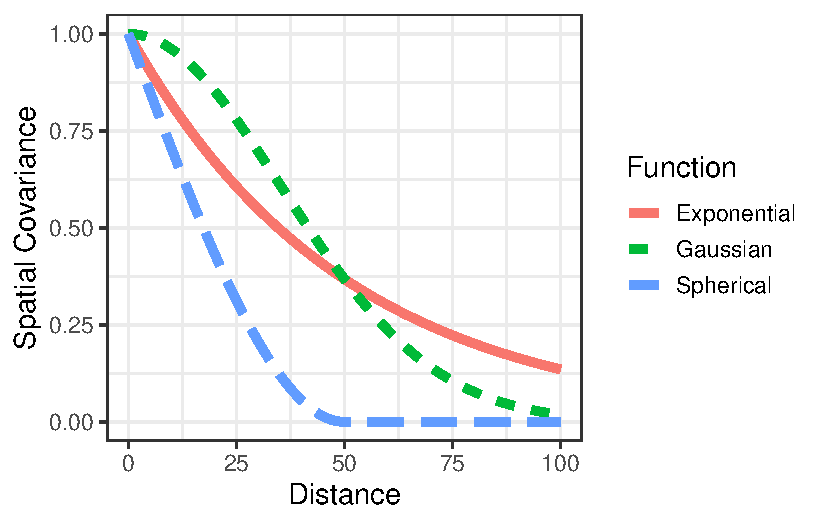
\includegraphics[width=0.75\linewidth,height=\textheight,keepaspectratio]{WBreport_files/figure-pdf/fig-spcov_fns-1.pdf}

}

\caption{\label{fig-spcov_fns}Three spatial covariance functions that
represent different spatial dependence behavior.}

\end{figure}%

Like the traditional linear model, the spatial linear model can capture
complex nonlinearities in the data through the use of interaction
effects \citep{faraway2002practical, lenth2025emmeans}, splines
\citep{chambers1992statistical, ruppert2003semiparametric}, additive
models \citep{wood2017generalized, pedersen2019hierarchical}, and
penalized regression models like the ridge and lasso
\citep{tibshirani1996regression}. Generally, this is accomplished by
leveraging \emph{basis functions} that break down nonlinear behavior
into a set of additive linear components that may include penalty terms
which guard against overfitting. Furthermore, there is no assumption
that \(y_i\) itself is normally distributed; rather, distributional
assumptions are placed on the random errors after incorporating the
slope parameters. This clarification implies the spatial (and
nonspatial) linear models can be quite effective at modeling a range of
data that are not normally distributed. For highly nonnormal data, tools
like generalized linear models, which we discuss later, can be helpful.
Finally, under general conditions, the slope parameters of the spatial
(and nonspatial) linear models are approximately normally distributed
with a large sample size (see \citet{casella2024statistical} for a
general justification via the Central Limit Theorem and
\citet{zhang2005towards} for nuances regarding spatial data). This is
beneficial because it justifies valid hypothesis testing on the slope
coefficients (often of primary ecological interest), no matter the
distribution of the data (given certain assumptions are satisfied).

One of the most useful applications of the spatial linear model is
predicting the response variable at unobserved locations. A very useful
spatial prediction method called Kriging has a rich theoretical
justification \citep{cressie1990origins, stein1999interpolation}.
Kriging is the spatial analogue to best linear unbiased prediction
(BLUP) for mixed models \citep{henderson1975best}. Via Kriging, the
spatial linear model produces BLUPs at each unobserved location of
interest, alongside prediction intervals to characterize uncertainty.
While useful, sometimes the goal is to create a BLUP for an entire
region of interest based on realized (i.e., observed) covariate values.
This technique, which builds upon the theoretical foundations of
Kriging, is called block Kriging
\citep{ver2002sampling, cressie2006block}. The intuition is to make
point predictions at a very dense grid in the study region and then
average these predictions, appropriately characterizing uncertainty.
Together, Kriging and block Kriging provide a complete set of tools for
spatial prediction, given the fit of a spatial linear model.

Spatial generalized linear models are an extension of spatial linear
models to highly nonnormal data
\citep{christensen2002bayesian, zhang2002estimation, diggle2007model, bonat2016practical}.
\citet{verhoef2024marginal} proposed a novel application of the Laplace
approximation to enable restricted maximum likelihood estimation of
spatial generalized linear models. This model formulation builds upon
Equation~\ref{eq-splm1} and is given by
\begin{equation}\phantomsection\label{eq-spglm1}{
g(\mu_i) = \beta_0 + \beta_1x_{1, i} + \beta_2x_{2, i} + ... + \beta_p x_{p, i} + \tau_i + \epsilon_i,
}\end{equation} where \(g(\mu_i)\) is a ``link function'' that links the
distribution of \(y_i\) to a linear function of its mean, \(\mu_i\).
Common link functions include the log link for count and skewed data and
the logit link for binomial and proportion data
(Table~\ref{tbl-glm-families}). Using the same argument as for spatial
linear models, nonspatial random effects can be added to spatial
generalized linear models.

\begin{table}

\caption{\label{tbl-glm-families}Common generalized linear model
families, link functions, and appropriate data types.}

\centering{

\centering
\begin{tabular}{llll}
  \toprule
Family & Link Function & Link Name & Data Type \\ 
  \midrule
Binomial & $f(\mu) = \log(\mu / (1 - \mu))$ & Logit & Binary; Binary Count \\ 
  Poisson & $f(\mu) = \log(\mu)$ & Log & Count \\ 
  Negative Binomial & $f(\mu) = \log(\mu)$ & Log & Count \\ 
  Beta & $f(\mu) = \log(\mu / (1 - \mu))$ & Logit & Proportion \\ 
  Gamma & $f(\mu) = \log(\mu)$ & Log & Skewed \\ 
  Inverse Gaussian & $f(\mu) = \log(\mu)$ & Log & Skewed \\ 
   \bottomrule
\end{tabular}

}

\end{table}%

Spatial models are complicated, both theoretically and computationally.
This has contributed to their relative underuse in the ecological
community. However, recent advances in open-source software have made
spatial models more accessible to ecologists who have strong subject
matter expertise but may lack sufficient statistical background or
computational skills to implement them from scratch. One such
advancement is the \texttt{spmodel} \textbf{R} package
\citep{dumelle2023spmodel}, which emulates base-\textbf{R} functions
like \texttt{lm()} and \texttt{glm()} to account for spatial dependence
via \texttt{splm()} and \texttt{spglm()}, respectively. Familiar
\textbf{R} functions like \texttt{summary()} and \texttt{predict()} can
be used directly on models fit via \texttt{spmodel}. Importantly,
\texttt{spmodel} also has tools for spatial random forest residual
modeling \citep{fox2020comparing}, applications to large data of several
thousand observations via spatial indexing \citep{ver2023indexing}, and
cross validation \citep{stone1974cross, roberts2017cross}.





\end{document}
